\chapter{METODE PENENILITIAN}

\setlength{\intextsep}{0cm}
% \setlength{\textfloatsep}{-1cm}

\section{Waktu dan Lokasi Penelitian}
Penelitian ini dilaksanakan dari bulan juli 2020 sampai dengan bulan november 2020. Lokasi penelitian dilakukan di Laboratorium Rekayasa Perangkat Lunak Fakultas Matematika dan Ilmu Pengetahuan Alam, Universitas Hasanuddin.

\section{Tahapan Penelitian}

\begin{table} [H]
    \begin{tabular}{|>{\centering\arraybackslash}m{1\linewidth} |}
        \hline
        \textbf{Analisis Kebutuhan}\\ 
        Pada tahapan ini merupakan tahap awal yaitu menganalisis semua kebutuhan yang diperlukan selama meneliti seperti pengumpulan teori terkait dengan penelitian yang terdapat dalam buku atau jurnal.\\
        \hline
    \end{tabular}
\end{table}

\begin{center}
    \bigg\downarrow
\end{center}

\begin{table} [H]
    \begin{tabular}{|>{\centering\arraybackslash}m{1\linewidth} |}
        \hline
        \textbf{Desain Sistem}\\ 
        Pada tahap ini dilakukan perancangan sistem yang akan dibangun seperti, rancangan sistem, rancangan skematik alat, \textit{use case} diagram, \textit{activity} diagram dan perancangan aplikasi web.\\
        \hline
    \end{tabular}
\end{table}

\begin{center}
    \bigg\downarrow
\end{center}

\begin{table} [H]
    \begin{tabular}{|>{\centering\arraybackslash}m{1\linewidth} |}
        \hline
        \textbf{Implementasi}\\ 
        Pada tahapan ini dilakukan implementasi dari hasil perancangan pada tahapan sebelumnya. Di tahapan inilah pembangunan sistem parkir, perangkaian sensor-sensor dan \textit{microcontoller} dilakukan.\\
        \hline
    \end{tabular}
\end{table}

\begin{center}
    \bigg\downarrow
\end{center}

\begin{table} [H]
    \begin{tabular}{|>{\centering\arraybackslash}m{1\linewidth} |}
        \hline
        \textbf{Pengujian Sistem}\\ 
        Pada tahapan ini hasil dari pembuatan sistem siap untuk diimplementasikan. Sensor ditempatkan di tempat yang sudah disediakan, maka alat ini akan mengumpulkan data yang dibutuhkan seperti nomor plat, id rfid, dan jarak ultrasonik. Data yang berhasil dikumpulkan akan disimpan di database dan bisa dilihat di web.\\
        \hline
    \end{tabular}
\end{table}

\begin{center}
    \bigg\downarrow
\end{center}

\begin{table} [H]
    \begin{tabular}{|>{\centering\arraybackslash}m{1\linewidth} |}
        \hline
        \textbf{Kesimpulan}\\ 
        Pada tahap ini merupakan tahap penting terakhir dari penelitian ini. Pada tahapan ini hasil dari pembuatan sistem parkir sudah siap untuk diimplementasikan.\\
        \hline
    \end{tabular}
\end{table}

\section{Sumber Data}
Sumber data dari penelitian ini menggunakan data primer yang didapatkan secara langsung dari sensor yang digunakan dalam sistem parkir.

\section{Rancangan Sistem}
Sensor dan kamera akan terhubung dengan raspberry pi. Berikut ini adalah gambaran mengenai rancangan dari penelitian ini :\newline

\begin{afigure} 
    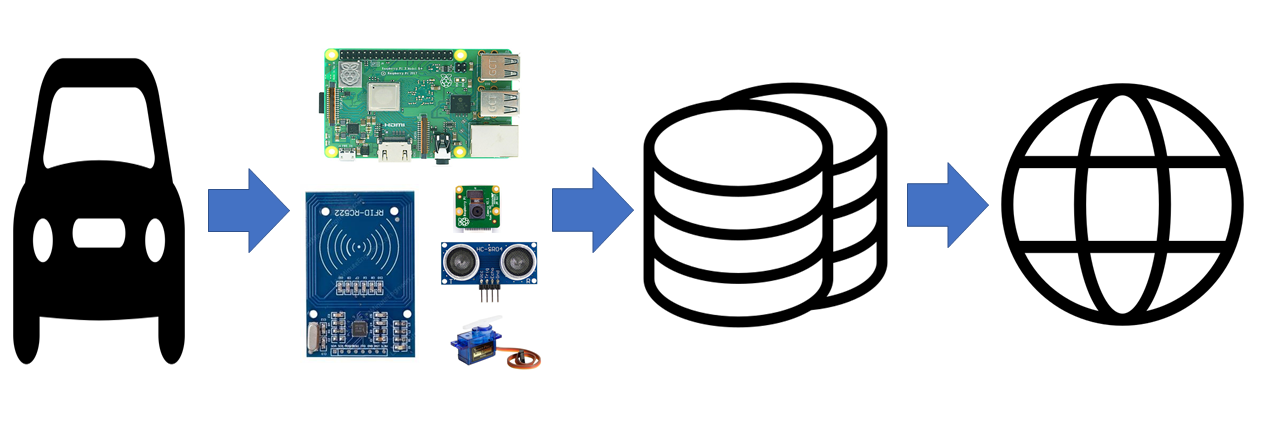
\includegraphics[width=0.85\textwidth, center]{images/rancangan sistem.png}
    \caption{Rancangan Sistem}
    \label{fig:RancanganSistem}
\end{afigure}

Pada gambar ~\ref{fig:RancanganSistem} saat pengemudi kendaraan menempelkan tag RFID mereka ke RFID reader, kamera pada raspberry akan mengambil gambar untuk di identifikasi nomor pelat tersebut. Hasil identifikasi akan berupa data nomor pelat kendaraan yang akan disimpan. Setelah itu servo yang berfungsi sebagai palang pintu akan terbuka. Data yang dikumpulkan oleh sensor berupa Id RFID dan nomor pelat kendaraan dapat dilihat melalui aplikasi web.

\section{Rancangan \textit{Use Case} Diagram}
Rancangan \textit{use case} diagram pada penelitian ini dapat di gambarkan seperti diagram dibawah ini:

\begin{afigure} 
    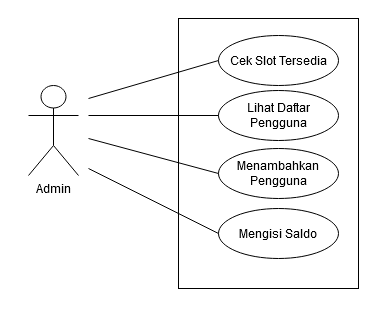
\includegraphics[width=0.85\textwidth, center]{images/Use Case Diagram.png}
    \caption{Use Case Diagram}
    \label{fig:usecasediagram}
\end{afigure}

sesuai dengan gambar ~\ref{fig:usecasediagram}, sistem yang akan dibangun hanya terdapat satu jenis akun yaitu akun admin yang akan mengawasi seluruh aktivitas pemarkiran melalui aplikasi web sebagai \textit{user interface}.

\section{Instrumen Penelitian}
Instrumen penelitian pada penelitian ini meliputi kebutuhan perangkat keras dan kebutuhan perangkat lunak.

\begin{enumerate}[topsep=0pt,itemsep=0pt,partopsep=0pt, parsep=0pt]
\item Kebutuhan perangkat keras
    \begin{itemize}[topsep=0pt,itemsep=0pt,partopsep=0pt, parsep=0pt,]
        \item Raspberry Pi
        \item Sensor RFID MFRC522
        \item Sensor Ultrasonik HC-SR04
        \item Servo SG90
        \item Camera Raspberry Pi v2 8mp
        \item Kabel Jumper
        \item Bread Board
        \item Memori Card
    \end{itemize}
\item Kebutuhan perangkat lunak
    \begin{itemize}[topsep=0pt,itemsep=0pt,partopsep=0pt, parsep=0pt,]
        \item \textit{Operating System (OS)} Raspbian
        \item \textit{Python Programming Language} (bahasa pemrograman yang digunakan)
        \item Visual Studio Code
        \item Web Browser
    \end{itemize}
\end{enumerate}